\documentclass[]{llncs} % "you can ignore this hint if your document works"
\usepackage{makeidx}
\usepackage{graphicx}
\usepackage{makecell}
\usepackage{float}
\begin{document}
\addtocmark{Southern Methodist University}

\title{Machine Learning Predicts Aperiodic Laboratory Earthquakes}
\author{Olha Tanyuk, Daniel Davieau, Charles South \and Daniel W. Engels}
\institute{Southern Methodist University, Dallas TX 75205, USA \newline otanyuk@mail.smu.edu, danieldavieau@mail.smu.edu, csouth@mail.smu.edu, dwe@lyle.smu.edu }


\maketitle
\begin{abstract}
In this paper we found the pattern of aperiodic seismic signals that precede earthquakes at any time in the earthquake’s cycle using a small window of time. We use data collected from a laboratory experiment which exhibits similar behavior to natural earthquakes, so the same approach may work in predicting the timing of natural earthquakes. We apply machine learning to a data set that comes from a classic laboratory experiment having several stick-slip displacements (earthquakes), a type of experiment which has been studied in depth as a simulation of seismologic faults for decades. We show that by listening to the acoustic signal emitted by the laboratory experiment a machine learning algorithm can predict the time remaining before it fails. These predictions are based only on the the acoustic signal and not its history. \par
	
%In this paper we present a method for predicting the timing of laboratory earthquakes using machine learning. If a similar approach can be applied to improve natural earthquake prediction it will save lives. We use data collected from a laboratory experiment which exhibits similar behavior to natural earthquakes. We train a machine learning algorithm using half of the data, then predict using the other half. We compare predicted versus actual timings to measure the algorithm's accuracy. The result shows that the timing of laboratory earthquakes can be predicted up to 16 seconds in advance with 71\% accuracy. The method and result demonstrates that machine learning can help if it can be scaled from the laboratory experiment to natural earthquakes. \par
\end{abstract}

\section{Introduction}
Earthquakes cause mass destruction and loss of life. A traditional method to predict earthquakes is to look to past recurrence intervals. Because the recurrences are not constant, predictions can only be made within broad time windows. One such model predicted that a strong earthquake would occur between 1985 and 1993 in the Parkfield California area but no significant event actually occurred until 2004 \cite{Jackson}. \par

Advances in instrumentation quality and density have fostered hope that progress can be made in forecasting. These advances have led to exciting discoveries of previously unidentified slip processes such as slow slips. Slow Slip Earthquakes (SSE) are fault behaviors that occur slowly enough to make them undetectable without instrumentation. They do not cause immediate widespread destruction like regular earthquakes do. They occur near the boundaries of large earthquake rupture zones \cite{Slip}. There is evidence to suggest that there is a relationship between slow slip earthquakes and more noticeable regular earthquakes \cite{SlowSlip}. \par

Researchers imitate natural slow slip earthquakes in the laboratory by placing rocky material between steel blocks and applying shear stress to induce slipping. Recent improvements in the instruments \cite{kaggle} used to measure signals have enabled the collection of larger volume data from more realistic and unpredictable laboratory earthquakes. However, processing the data and detecting patterns in it has become more difficult to work with. In this paper we demonstrate that machine learning can be used to detect patterns in the more realistic data and predict laboratory earthquakes. \par

In this paper, given seismic signal data with considerably more aperiodic slow-slip laboratory earthquake failures, we find the pattern of acoustic signals to predict the time at which laboratory earthquakes will occur at any time in the slip cycle. \par

We use acoustic data provided by the Los Alamos National Laboratory (LANL) as part of a 2019 Kaggle competition \cite{kaggle}, which also represents laboratory slow-slip earthquakes. The data is very aperiodic and more realistic than the data LANL studied earlier in 2017. \cite{kaggle}. The results of this experiment are potentially applicable to the field of real world earthquakes \cite{Bertrand}. Other potential applications include avalanche prediction or failure of machine parts \cite{Bertrand}. \par


%Earthquakes cause mass destruction and loss of life. Traditional earthquake prediction methods have relied on recurrence interval based models. Because the recurrences are not constant predictions can only be made within decade spanning time windows. One such model predicted that a magnitude 6 earthquake would occur between 1985 and 1993 in the Parkfield California area but no significant event occurred until 2004 \cite{Jackson}. \par
%
%Researchers imitate natural earthquakes in the laboratory by placing rocky material between steel blocks and applying shear stress to induce slipping. Recent improvements in the instruments \cite{Bertrand} used to measure signals have enabled the collection of larger volume data from more realistic and unpredictable laboratory earthquakes. However processing the data and detecting patterns in it has become more difficult to work with. In this paper we demonstrate that machine learning can be used to detect patterns and make predictions from realistic, unpredictable laboratory earthquake data \cite{kaggle}.\par
%
%We use data which was collected by the Los Alamos National Laboratory and provided to the public via a Kaggle competition \cite{kaggle}. It consists of 629 million acoustic signal observations and an accompanying record of the time remaining until a laboratory earthquake (failure) occurred \cite{Bertrand}. We calculate additional statistical measures such as variance, kurtosis and skew for each observation. We use half of the data to train a machine learning algorithm. With the remaining half of the data, using only the acoustic signal as input we calculate a prediction of the time remaining until failure. We measure  accuracy by comparing the predicted to actual remaining time to failure from the original data. \par
%
%The result shows that the timing of laboratory earthquakes can be predicted up to 16 seconds in advance with 71 percent accuracy.\par
%
%%Conclusion
%The data, hardware and software allows us to predict impending earthquakes. However we only know 8-16 seconds before failure. Therefore practical applications may be limited. This may prove useful but only applies to laboratory experiments. This could be used in industry perhaps in researching materials for wallboard, machine parts and others.\par

\section{Background}
\subsection{Statistical Values to Evaluate Predictions}
\begin{figure}
	\centering
	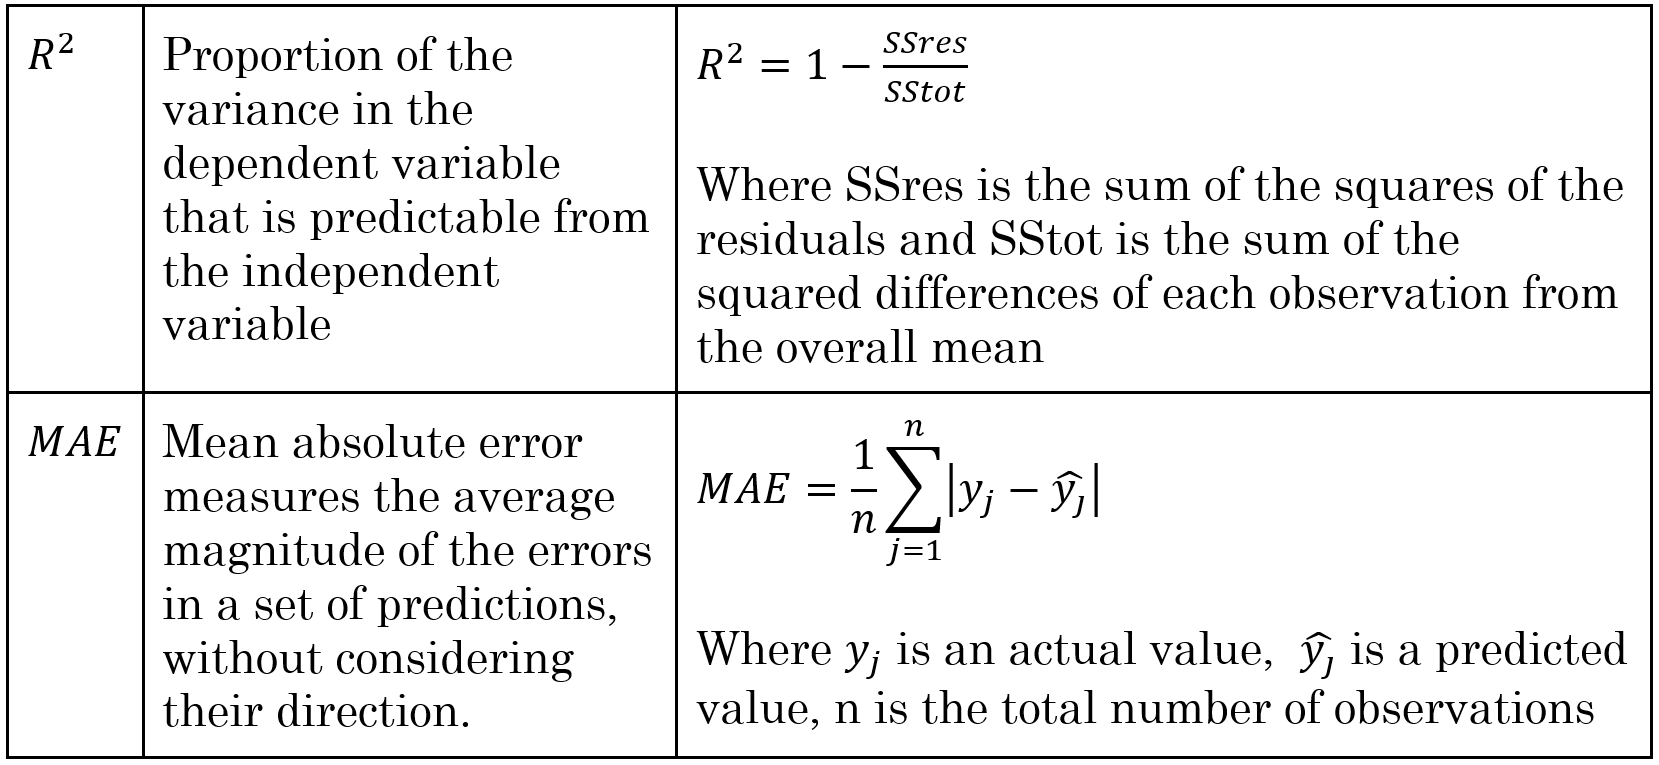
\includegraphics[width=.9\linewidth]{background}
	\caption{The values used to evaluate predictions in our work are the coefficient of determination $r^2$ and mean absolute error ($MAE$).}
	\label{fig:background}
\end{figure}

\subsection{Earthquakes}
An earthquake is the shaking of the surface of the Earth, resulting from the sudden release of energy in the Earth’s lithosphere that creates seismic waves [11]. It  happens when two blocks of the earth suddenly slip past one another. The surface where they slip is called the fault or fault plane [12].\par
The earth has four major layers: the inner core, outer core, mantle and crust [12]. The crust and the top of the mantle make up a thin skin on the surface of our planet; this skin is not all in one piece – it is made up of many pieces like a puzzle covering the surface of the earth [12]. These puzzle pieces are called tectonic plates, and the edges of the plates are called the plate boundaries.  Tectonic plates  keep slowly moving around, sliding past one another and bumping into each other. The plate boundaries are made up of many faults, and most of the earthquakes around the world occur on these faults[12]. Since the edges of the plates are rough, they get stuck while the rest of the plate keeps moving [12]. Finally, when the plate has moved far enough, the edges unstick on one of the faults and there is an earthquake [12]. \par
The size of an earthquake depends on the size of the fault and the amount of slip on the fault, but that’s not something scientists can simply measure with a measuring tape since faults are many kilometers deep beneath the earth’s surface [12]. The size of the earthquake is called its magnitude. The Richter Scale (ML) is what most people have heard about, but in practice it is not commonly used anymore, except for small earthquakes recorded locally, for which ML and short-period surface wave magnitude (Mblg) are the only magnitudes that can be measured [13]. For all other earthquakes, the moment magnitude (Mw) scale is a more accurate measure of the earthquake size [13]. 


\subsection{Los Alamos National Laboratory's Findings}
In 2017 Los Alamos National Laboratory (LANL) researchers discovered a way to successfully predict Slow Slip Earthquakes (SSE) in a laboratory experiment that simulates natural conditions. The team trained a computer to pinpoint and analyze quasi‐periodic seismic and acoustic signals emitted during the movements along the fault. They processed massive amounts of data and identified a particular sound pattern previously thought to be noise that precedes an earthquake. The team was able to characterize the time remaining before a laboratory earthquake at all times using a time window of 1.8 sec of the data to make each prediction with 89\% coefficient of determination \cite{LANLNews}. This result was achieved using a Random Forest Regression machine learning technique and quasi‐periodic data. \par

In the lab, the team imitated a real earthquake using steel blocks interacting with rocky material to cause slipping that emitted seismic sounds. An accelerometer recorded the acoustic emission emanating from the sheared layers \cite{LANLNews}. For the first time, researchers discovered a pattern that accurately predicted when a laboratory earthquake would occur. The LANL team acknowledges that the characteristics of the lab experiment such as shear stress differ from natural earthquakes but the application of the analysis to the real world to validate their results is ongoing. This method can also be applied outside of seismology to support material failure research in other fields such as aerospace and energy \cite{LANLNews}. The lab results reveal that the fault does not fail randomly but in a predictable manner. The observations also demonstrate that the fault’s critical stress state which indicates when it might slip can be determined using exclusively an equation of state \cite{LANLNews}. So far seismologists and earth scientists have mostly relied on catalogs of historical data to try to characterize the state of faults. These catalogs contain a minute fraction of seismic data with portions discarded during analysis as useless noise. The authors discovered that hidden in the noise-like data are signals that inform them of the state of the fault much more precisely than catalogs \cite{LANLNews}. \par
\subsection{Experimental Setup}
The laboratory system is a two‐fault configuration that contains fault gouge material submitted to double direct shear \cite{kaggle}. \par
\begin{figure}[h]
	\centering
	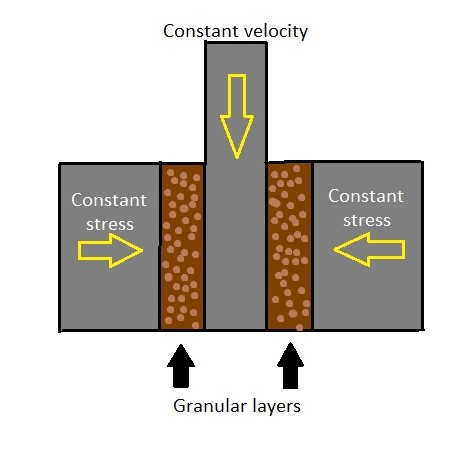
\includegraphics[width=.6\linewidth]{lab}
	\caption{Classic laboratory earthquake model }
	\label{fig:lab}
\end{figure}
Two fault gouge layers are sheared simultaneously while subjected to a constant normal load and a prescribed shear velocity \cite{kaggle}. The laboratory faults fail in repetitive cycles of stick and slip that is meant to mimic the cycle of loading and failure on tectonic faults \cite{kaggle}. While the experiment is considerably simpler than a fault in the Earth it shares many physical characteristics \cite{kaggle}. \par

A driving piston displaces at a very constant velocity during the inter-event time and accelerates briefly when a slip occurs \cite{Bertrand}. An accelerometer records the acoustic emission emanating from the shearing layers \cite{Bertrand}. The steel blocks are extremely stiff therefore the deformation takes place largely in the gouge \cite{Bertrand}. Under a broad range of load and shear velocity conditions, the apparatus stick‐slips quasi‐periodically for hundreds of stress cycles during a single experiment and in general follows predictions from rate and state friction \cite{Bertrand}. The rate of impulsive precursors accelerates as failure approaches suggesting that upcoming laboratory earthquake timing could be predicted \cite{Bertrand}. \par

The experimental data has 16 earthquakes. The shortest time to failure is 1.5 seconds for the first earthquake, 7 seconds for the 7th and the longest is around 16 seconds. \par

\subsection{Random Forest Regressor Overview}
The random forests (RF) algorithm is as follows:\par
1. Draw n(tree) bootstrap samples from the original data [10].\par
2. For each of the bootstrap samples, grow an unpruned regression tree, with the following modification: at each node, rather than choosing the best split among all predictors, randomly sample m(try) of the predictors and choose the best split from among those variables [10].\par
3. Predict new data by aggregating the predictions of the n(tree) trees [10].\par
In our work the training data is used to generate the RF model. The testing data is used to evaluate the performance of the RF model; this constitutes a fair measure of the RF performance because the testing data is independent from the training process (i.e. out of sample performance). It is very important to ensure that testing data does not leak into the training process [5]. \par
The tree is given by a bootstrap resampling of the training data, which induces variation between the trees and mitigates the effect of outliers on the forest [5]. To generate each node, we formulate a "yes"/"no" decision (corresponding to a split into left/right branches) operating on the data available at the current node. At each node, we select a random subset of the available features. From the selected features, we construct the decision that best predicts the time to failure [5].


\section{Data} 
The data used in this work is a 157.275 second recording of seismic signals (ordered sequentially.) It was recorded at 4MHz hence 629,145,480 data points accompanied by the time remaining in seconds until the following lab earthquake. \par
The seismic signals are recorded using a piezoceramic sensor which outputs a voltage upon deformation by incoming seismic waves (henceforth we will use the term acoustic signal). The seismic data, which serves as the input to our analysis, is this recorded voltage, in integers. \par
% to prevent images from floating all over the place in the document: https://tex.stackexchange.com/questions/16207/image-from-includegraphics-showing-up-in-wrong-location
%\begin{table}
%	\begin{center}
%		\caption{Data Definitions}
%		\label{tab:DataDefinitions}
%		\begin{tabular}{ll}
%			\textbf{Acoustic Signal} & Voltage upon deformation by incoming seismic waves. \\
%			\textbf{Time To Failure} & The remaining time in seconds until an actual stick-slip failure occurred.  \\
%		\end{tabular}
%	\end{center}
%\end{table}
Acoustic signal is voltage upon deformation by incoming seismic waves. \par
Time to failure is the remaining time in seconds until an actual stick-slip failure occurred. \par

\begin{table}
	\begin{center}
		\caption{}
		\label{tab:SampleData}
		\begin{tabular}{c|r} 
			\textbf{Acoustic Signal} & \textbf{Time to Failure}\\
			\hline
			12 & 1.469099998474121 \\ 
			6 & 1.469099998474121 \\ 
			8 & 1.469099998474121 \\ 
			5 & 1.469099998474121 \\ 
			8 & 1.469099998474121 \\ 
		\end{tabular}
	\end{center}
\end{table}
\begin{figure}
	\centering
	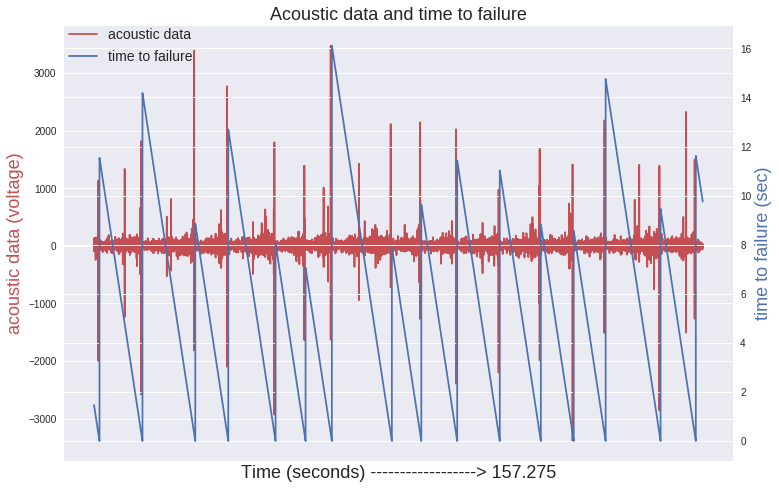
\includegraphics[width=.9\linewidth]{timeSeries}
	\caption{We can see that the acoustic signal shows huge fluctuations regularly just before the failure. It is also worth noting that failures can be predicted visually as cases when huge fluctuations in the signal are followed by smaller signals.}
	\label{fig:timeseries}
\end{figure}
\begin{figure}
	\centering
	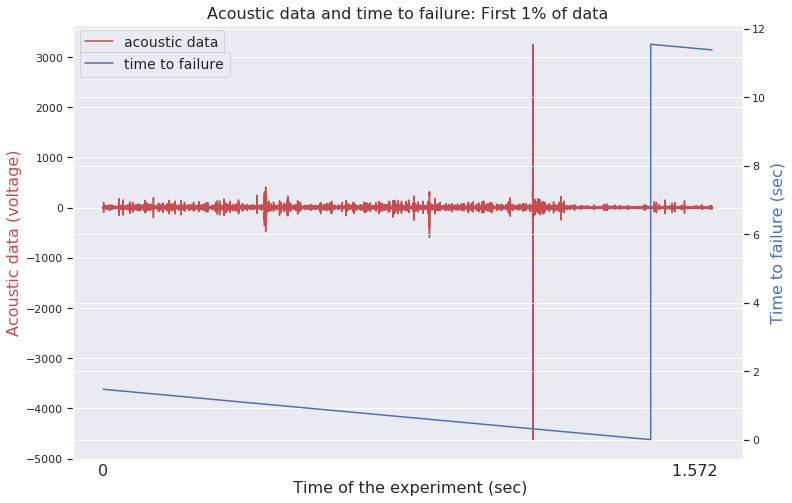
\includegraphics[width=.9\linewidth]{zoomedInTimePLot}
	\caption{On this zoomed-in time plot we can see that the large acoustic signal oscillation at the 1.572 second mark is not at the exact time of the failure but  just before it. There are trains of intense signal oscillations preceding the large one and some smaller ones after it.}
	\label{fig:zoomeInTimePlot}
\end{figure}
\begin{figure}
	\centering
	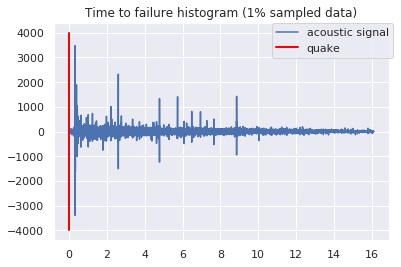
\includegraphics[width=.8\linewidth]{timeToFailureHistogram}
	\caption{In this 1\% sample of the data we can see that the voltage amplitude of acoustic precursors accelerates as failure approaches, suggesting that upcoming laboratory earthquake timing could be predicted. The red line indicates that a quake occurs when the time to failure approaches 0. The minimum time remaining until the quake is -5.5150e+03 sec.}
	\label{fig:timeToFailureHistogram}
\end{figure}
\begin{figure}
	\centering
	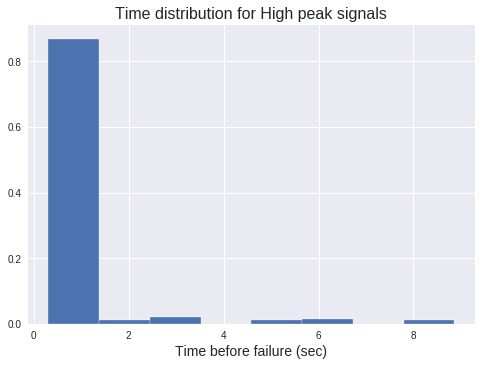
\includegraphics[width=.8\linewidth]{timeDistribution}
	\caption{We found that more than 90\% of high acoustic signal values (absolute value greater than 1000) are around 0.31 seconds before an earthquake.}
	\label{fig:timeDistribution}
\end{figure}
\begin{figure}
	\centering
	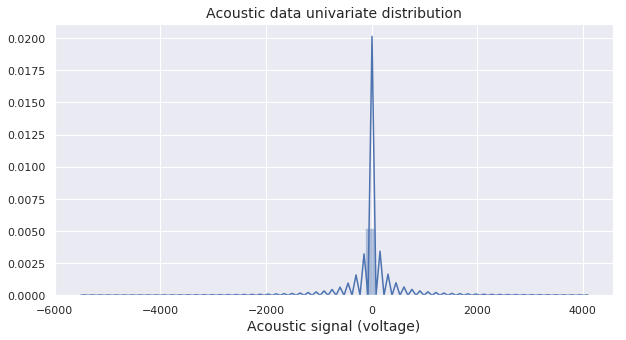
\includegraphics[width=.9\linewidth]{acousticDataDistribution}
	\caption{The distribution of the acoustic signals have a very high peak and we see outliers in both directions}
	\label{fig:acousticDataDistribution}
\end{figure}
\begin{figure}
	\centering
	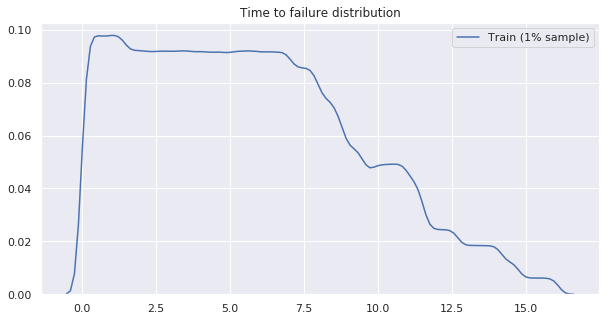
\includegraphics[width=.9\linewidth]{timeToFailureDistribution}
	\caption{The distribution of the time to failure is right skewed. We evaluated model performance using normalized and not normalized distribution of the time to failure.}
	\label{fig:timeToFailureDistribution}
\end{figure}
\begin{figure}
	\centering
	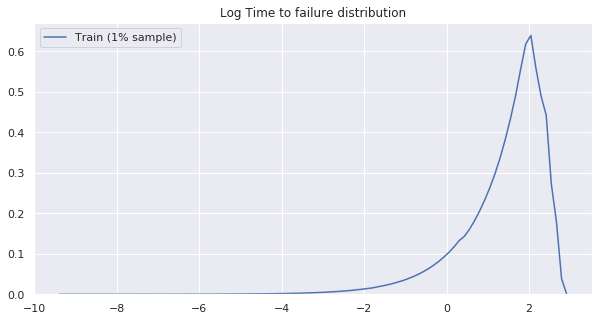
\includegraphics[width=.9\linewidth]{logTimeToFailureDistribution}
	\caption{In this plot we can see that applying a logarithmic transform to the time to failure results in a left skewed distribution.}
	\label{fig:logTimeToFailureDistribution}
\end{figure}
\begin{figure}
	\centering
	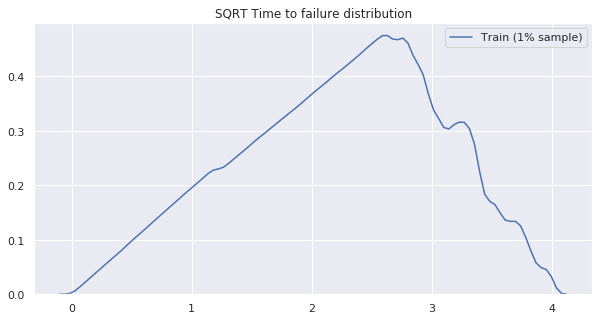
\includegraphics[width=.9\linewidth]{sqrtTimeToFailureDistribution}
	\caption{In this plot we can see that applying a square root transformation to the time to failure is still not normal but improved the distribution significantly. We used a square root transformation for normalization of the time to failure distribution.}
	\label{fig:sqrtTimeToFailureDistribution}
\end{figure}
\clearpage
\newpage
\section{Feature Engineering}
Working with quasi periodic seismic signals LANL achieved a 0.89 coefficient of determination. They divided the data into 1.8 second time windows and used a Random Forest technique. \cite{Bertrand}. The most important features in the LANL model were variance, kurtosis and threshold. \par
We used a similar approach in this study. Our goal is to predict the time remaining before the next failure using only moving time windows of the acoustic data. We divided the data into 0.3 second time windows (1,500,000 observations) which is small enough relative to the lab quake cycle which spans 8 to 16 seconds. As indicated in figure 6 more than 90\% of high acoustic values (absolute value greater than 1000) are around 0.31 seconds before an earthquake. It makes sense to divide our data by 0.3 sec windows to reduce error at the end of the quake cycle. 

\begin{figure}
	\centering
	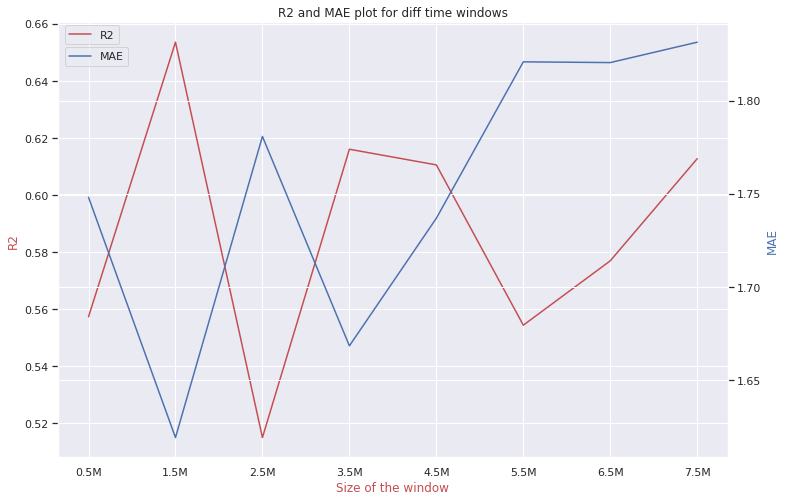
\includegraphics[width=.9\linewidth]{rSquaredandMAE}
	\caption{Checking how sensitive our results are to the size of the time window we find that the highest $r^2$ and smallest mean absolute error we were able to achieve is with 1.5M observations in each time window.}
	\label{fig:rSquaredandMAE}
\end{figure}

Our resulting transformed data set consists of 419 time windows (0.3 seconds each).  From each time window we compute a set of 95 potentially relevant statistical features (e.g., mean, variance, kurtosis, min/max, threshold and so on). Using feature importance techniques we found that only the following (in Table 3) are considerably important:
\begin{table}[H]
	\begin{center}
		\caption{List of Engineered Features}
		\label{tab:engineeredFeatrures}
		\begin{tabular}{l} 
Standard Deviation \\
90\% Quantile \\
95\% Quantile \\
99\% Quantile \\
Absolute Standard Deviation \\
Average Rolling Standard Deviation for 100, 1000 and 10000 observations \\
Variance of Rolling Standard Deviation for 100, 1000 and 10000 observations \\
Minimum Rolling Standard Deviation for 100, 1000 and 10000 observations \\
1\% Quantile of rolling standard deviation for 100, 1000, 10000 observations \\
5\% Quantile of rolling standard deviation for 100, 1000, 10000 observations \\
10\% Quantile of rolling standard deviation for 100, 1000, 10000 observations \\
90\% Quantile of rolling standard deviation for 100, 1000, 10000 observations \\
95\% Quantile of rolling standard deviation for 100, 1000, 10000 observations \\
99\% Quantile of rolling standard deviation for 100, 1000, 10000 observations \\
Variance of Rolling Absolute Mean for 100, 1000 and 10000 observations \\
		\end{tabular}
	\end{center}
\end{table}

We apply different machine learning techniques such as the Random Forest Regressor, XGB Regressor,  Decision Tree Regressor, LGBM Regressor and Extra Trees Regressor to the new continuous values that we created analyzing acoustic time series data. \par
To avoid correlation between the new features we applied a principal component analysis technique. The principle components allows us to reduce the number of features from 35 to only 5 which represents 99.9\% of the full data variation. \par
We use a 50/50 continuous split of the data for use as training and testing data sets respectively. Contiguity of the train and test data sets is important to minimize contamination of the training data with information about the test data. \par
We selected regularization hyper-parameters for each machine learning algorithm using random grid search technique based on a 3-fold cross-validation.
%\clearpage
%\newpage
\section{Results}
We run different techniques on a training data set (50\% of the full data) before principal component analysis and after. Principal component analysis did not allow for any significant improvement in our results. We apply our model to generate predictions on the test data  and measure the accuracy of them using $r^2$ (the coefficient of determination) and MAE (mean absolute error). \par 

The most accurate results were achieved by the Random Forest Regressor algorithm with 1,62 seconds MAE and 0.64 $r^2$. The parameters used are displayed in table 3. %Add Scitkitlearn definitions? Add top background definitions as well? 
The hyper-parameters used with the algorithm  were:

\begin{table}
	\begin{center}
		\caption{Extra Trees Regressor Parameters}
		\label{tab:hyperparameters}
		\begin{tabular}{l|l} 
			\textbf{Parameter} & \textbf{Setting}\\
			\hline
			Maximum Depth & 8 \\ 
			Maximum Features & log2 \\ 
			Minimum Samples Leaf & 2 \\ 
			Minimum Samples Split & 6 \\ 
			Number of Estimators & 1000 \\
		\end{tabular}
	\end{center}
\end{table}

\par

\begin{figure}
	\centering
	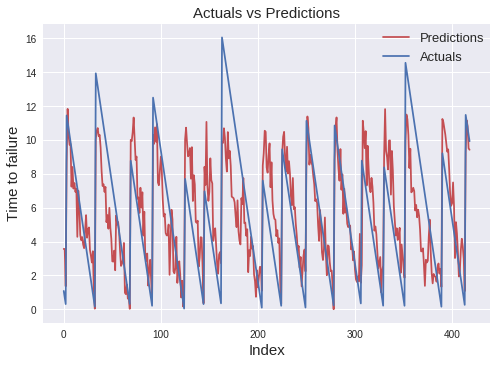
\includegraphics[width=.9\linewidth]{results1}
	\caption{We emphasize that there is no past or future information considered in calculating the predictions (red line). Each prediction uses only the acoustic signal information within one single time window.}
	\label{fig:results1}
\end{figure}

\begin{figure}[H]
	\centering
	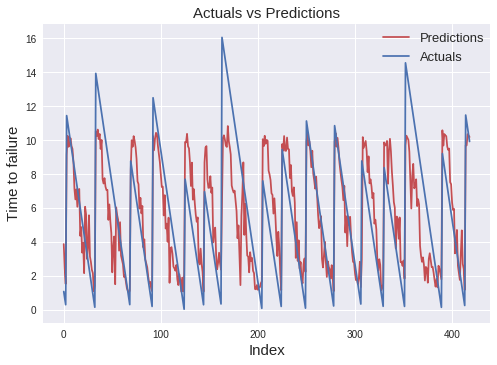
\includegraphics[width=.9\linewidth]{results2}
	\caption{Results achieved with the Ada Boost Regressor algorithm are 1.67 MAE and 0.62 $r^2$ score. The hyper parameters used are learning rate = 0.01826, loss = square, number of estimators = 500 and base estimator= Ridge(alpha=1).}
	\label{fig:results2}
\end{figure}
\clearpage
\newpage
\section{Analysis}
The most accurate results with coefficient of determination 0.65 and mean absolute error 1.61 seconds we achieved using the Extra Trees Regressor. The most important features are shown on figure 14. The top 5 are 90\% and 95\% quartile rolling standard deviations, standard deviation of rolling absolute mean and average rolling standard deviation.
%$SD = \sqrt{\frac{1}{N-1} \sum_{i=1}^N (x_i - \overline{x})^2}$
\begin{figure}[H]
	\centering
%	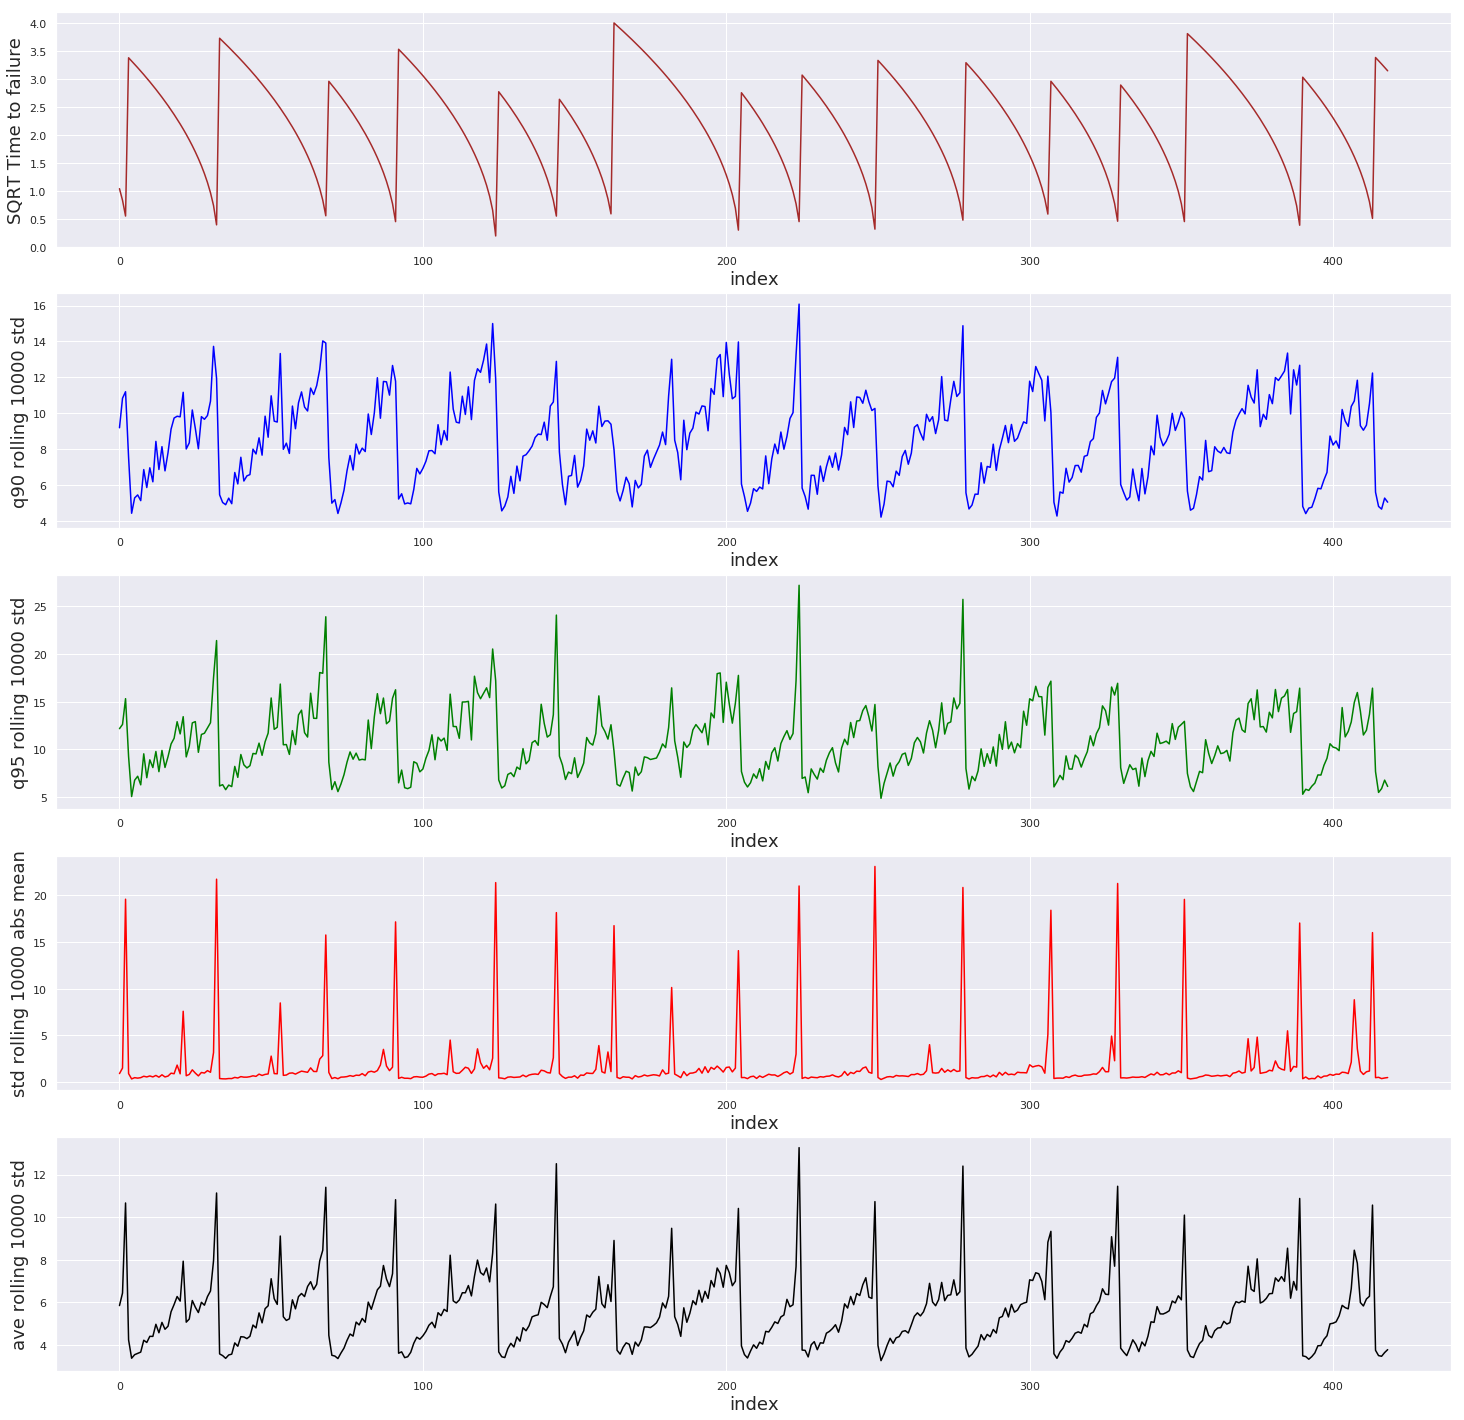
\includegraphics[width=14cm,height=14cm,keepaspectratio]{analysis}
	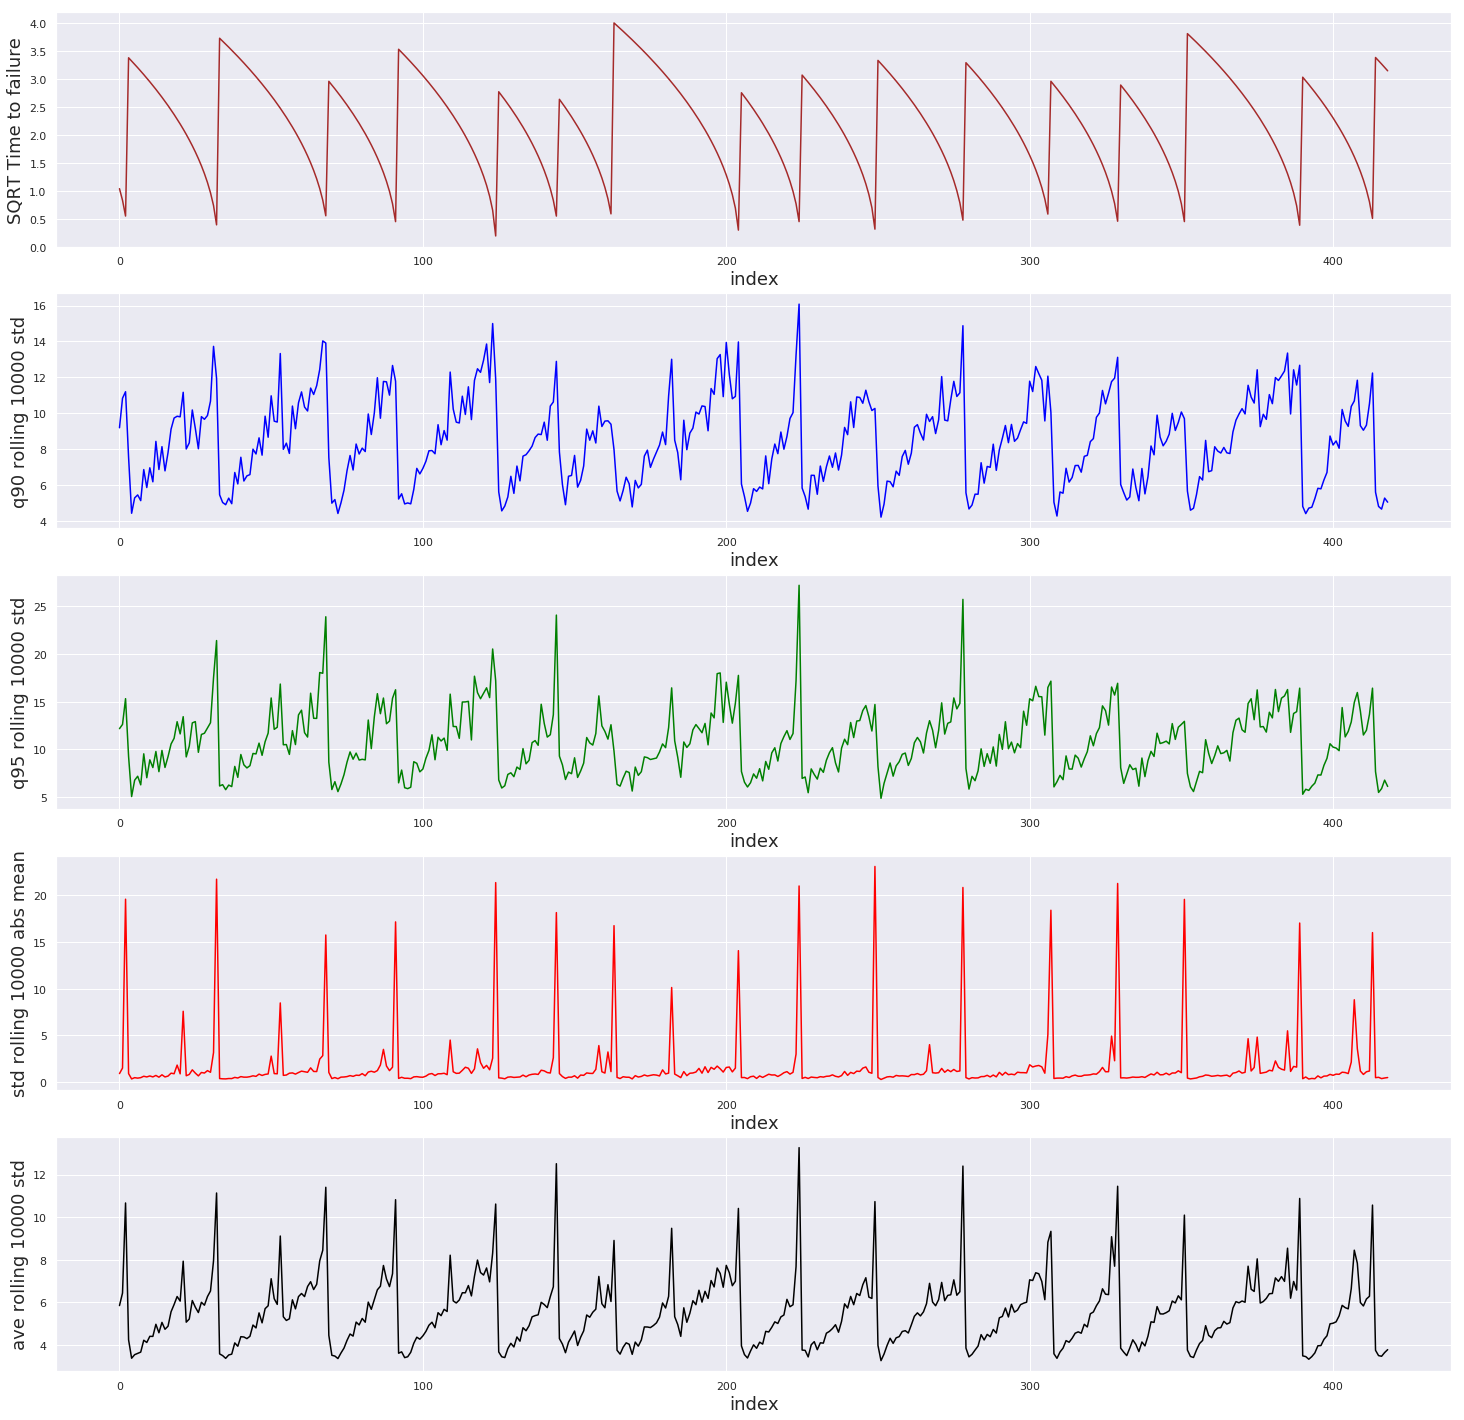
\includegraphics[width=1\linewidth]{analysis}
	\caption{}
	\label{fig:analysis}
\end{figure}

\section{Ethics}

Our responsibility to report our results has to be weighed with our responsibility not to cause social disturbance. If the method demonstrated in this paper is scaled and applied to predict natural earthquakes this balance must be considered. Unwarranted predictions could have affects on personal property value while failure to report warranted predictions could result in loss of life or avoidable property damage. \par

Clarence R. Allen, the chairman of the National Earthquake Prediction Evaluation Council claimed that keeping information, from the public and discussing hypotheses on earthquake prediction “behind closed doors” would cause more harm than good, for free speech is the only means to promote research and to increase public responsibility of scientists \cite{Ayhan}. The public’s demand for accurate information would encourage scientists to further their research and hinder them from making unwarranted statements that may cause disturbance in society \cite{Ayhan}. Allen seems to suggest that free scientific communication in its due course would bring order to the scientific environment by eliminating unwarranted scientific hypotheses and predictions, together with the guesses of amateurs and cranks \cite{Ayhan}.

In this study, we followed principles of the Association for Computing Machinery (ACM) Code of Ethics and Professional Conduct [https://www.acm.org/code-of-ethics] to ensure both privacy and security of individuals, and other codes of conducts related to good ethical practices. Ethical principles to make no harm, be honest and trustworthy, respect the work required to produce new ideas were used in our work. We also took professional responsibilities to achieve high quality in both the processes and professional work, maintain high standards of professional competence, accept and provide appropriate professional review, know and respect existing rules pertaining to professional work.

\section{Conclusions}

Given the more realistic data Machine Learning can provide failure forecasts based on small windows of time. The acoustic signal measurement is an indicator of imminent failure. The prior recurrence interval is not needed to make a prediction. The Extra Trees Regressor machine learning technique provides the most accurate results.

%The results are another step toward learning the siesmic signals encouraging Machine Learning analysis of seismic signals in Earth.


%The results show that laboratory earthquakes can be predicted up to 16 seconds in advance.  \par
%
In this study we are using only 157 seconds of data. Future work should introduce higher volumes of data to determine if accuracy can be improved. Also the combination of the acoustic signal and the recurrence interval should be tested to determine it's affect on accuracy.
\par

\section{Acknowledgment}
This research was supported by Dr. Michael L. Blanpied,  U.S. Geological Survey. We thank Dr. Michael L. Blanpied for comments that greatly improved our work.

%References
\bibliographystyle{splncs}
\bibliography{myBibliography}

\end{document}
